% TODO:
%   urgent queue (best maxTip) : floating queue (best maxFee) = 4 : 1
%   unit slot (32k bytes)
\begin{frame}[fragile]{mempool, a.k.a. \href{https://www.paradigm.xyz/2020/08/ethereum-is-a-dark-forest}{Dark Forest}}
  \begin{center}\makebox[0pt]{\scalebox{1.0}{% centering wide picture
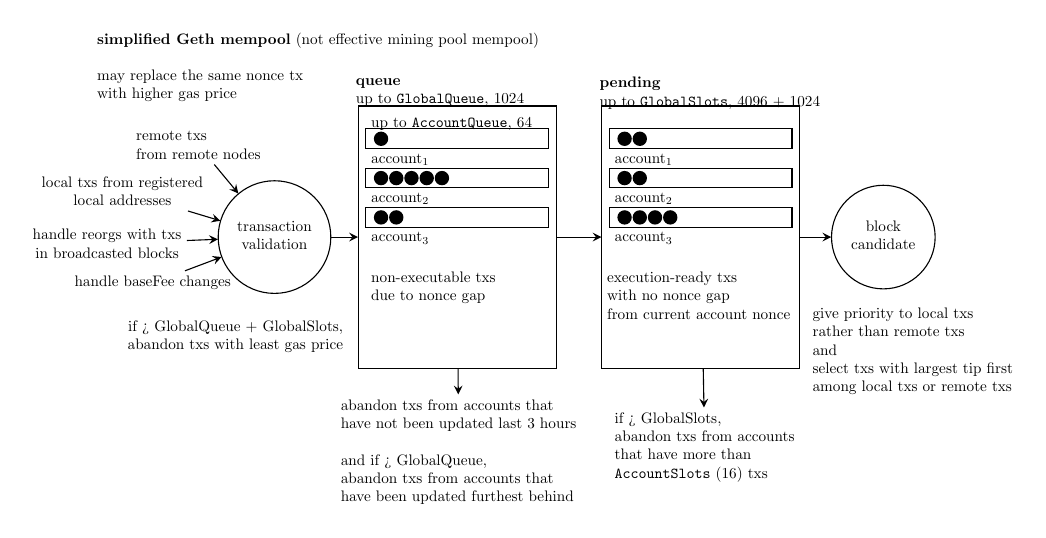
\begin{tikzpicture}[scale=0.55,every node/.style={transform shape}]
\def\hs{13em}
\def\vs{20ex}
\def\hh{3em}

\node[align=left,anchor=north west] at (-12em,32ex) {\textbf{simplified Geth mempool} (not effective mining pool mempool)\\\\may replace the same nonce tx\\with higher gas price};

\node[circle,draw] at (0em,0ex) (A) {\begin{tabular}{c}transaction\\validation\end{tabular}};
\node (B) at (\hs-1em,0ex) [draw,minimum width=\hs,minimum height=2*\vs] {};
\node (C) at (\hs+\hh+\hs-1em,0ex) [draw,minimum width=\hs,minimum height=2*\vs] {};
\node[circle,draw] at (\hs+\hh+\hs+\hs-2em,0ex) (D) {\begin{tabular}{c}block\\candidate\end{tabular}};

\node[align=left] (S1) at (-5em, 14ex) {remote txs\\from remote nodes};
\node[align=center] (S2) at (-10em, 7ex) {local txs from registered\\local addresses};
\node[align=center] (S3) at (-11em, -1ex) {handle reorgs with txs\\in broadcasted blocks};
\node[align=center] (S4) at (-8em, -7ex) {handle baseFee changes};

\draw[-stealth] (A) -- (B);
\draw[-stealth] (B) -- (C);
\draw[-stealth] (C) -- (D);
\draw[-stealth] (S1) -- (A);
\draw[-stealth] (S2) -- (A);
\draw[-stealth] (S3) -- (A);
\draw[-stealth] (S4) -- (A);

%\node[align=right,anchor=north west] at (-10em,16ex) {may replace the same nonce tx\\with higher gas price};
\node[align=right,anchor=north west] at (-10em,-12ex) {if > GlobalQueue + GlobalSlots,\\abandon txs with least gas price};
\node[align=left,anchor=north west] at (35em,-10ex) {give priority to local txs\\rather than remote txs\\and\\select txs with largest tip first\\among local txs or remote txs};

% decorate B
\node[align=left,anchor=north west] at (0.5*\hs-1.5em,\vs+5ex) {\textbf{queue}\\up to \texttt{GlobalQueue}, 1024};
\node[align=left,anchor=north west] at (0.5*\hs-0.5em,\vs-1ex) {up to \texttt{AccountQueue}, 64};
\node at (\hs-1em,\vs-5ex) [draw,minimum width=\hs-1em,minimum height=3ex] {};
\node[align=left,anchor=north west] at (0.5*\hs-0.5em,\vs-6.5ex) {account\textsubscript{1}};
\node[circle,fill] at (0.5*\hs+0.5em+0*1em,\vs-6.5ex+1.5ex-0*6ex) {};
\node at (\hs-1em,\vs-5ex-1*6ex) [draw,minimum width=\hs-1em,minimum height=3ex] {};
\node[align=left,anchor=north west] at (0.5*\hs-0.5em,\vs-6.5ex-1*6ex) {account\textsubscript{2}};
\node[circle,fill] at (0.5*\hs+0.5em+0*1em,\vs-6.5ex+1.5ex-1*6ex) {};
\node[circle,fill] at (0.5*\hs+0.5em+1*1em,\vs-6.5ex+1.5ex-1*6ex) {};
\node[circle,fill] at (0.5*\hs+0.5em+2*1em,\vs-6.5ex+1.5ex-1*6ex) {};
\node[circle,fill] at (0.5*\hs+0.5em+3*1em,\vs-6.5ex+1.5ex-1*6ex) {};
\node[circle,fill] at (0.5*\hs+0.5em+4*1em,\vs-6.5ex+1.5ex-1*6ex) {};
\node at (\hs-1em,\vs-5ex-2*6ex) [draw,minimum width=\hs-1em,minimum height=3ex] {};
\node[align=left,anchor=north west] at (0.5*\hs-0.5em,\vs-6.5ex-2*6ex) {account\textsubscript{3}};
\node[circle,fill] at (0.5*\hs+0.5em+0*1em,\vs-6.5ex+1.5ex-2*6ex) {};
\node[circle,fill] at (0.5*\hs+0.5em+1*1em,\vs-6.5ex+1.5ex-2*6ex) {};
\node[align=left,anchor=north west] at (0.5*\hs-0.5em,\vs-6.5ex-3*6ex) {non-executable txs\\due to nonce gap};
\node[align=left,anchor=north west] (B') at (0.5*\hs-1.5em+0.5em-1.5em,-\vs-6ex+2ex) {abandon txs from accounts that\\have not been updated last 3 hours\\\\and if > GlobalQueue,\\abandon txs from accounts that\\have been updated furthest behind};
\draw[-stealth] (B) -- (B');

% decorate C
\node[align=left,anchor=north west] at (1.5*\hs+\hh-1.5em,\vs+5.2ex) {\textbf{pending}\\up to \texttt{GlobalSlots}, 4096 + 1024};
%\node[align=left,anchor=north west] at (1.5*\hs+\hh-0.5em,\vs-1ex) {up to \texttt{AccountSlots}, 16};
\node at (2*\hs+\hh-1em,\vs-5ex) [draw,minimum width=\hs-1em,minimum height=3ex] {};
\node[align=left,anchor=north west] at (1.5*\hs+\hh-0.5em,\vs-6.5ex) {account\textsubscript{1}};
\node[circle,fill] at (1.5*\hs+\hh+0.5em+0*1em,\vs-6.5ex+1.5ex-0*6ex) {};
\node[circle,fill] at (1.5*\hs+\hh+0.5em+1*1em,\vs-6.5ex+1.5ex-0*6ex) {};
\node at (2*\hs+\hh-1em,\vs-5ex-1*6ex) [draw,minimum width=\hs-1em,minimum height=3ex] {};
\node[align=left,anchor=north west] at (1.5*\hs+\hh-0.5em,\vs-6.5ex-1*6ex) {account\textsubscript{2}};
\node[circle,fill] at (1.5*\hs+\hh+0.5em+0*1em,\vs-6.5ex+1.5ex-1*6ex) {};
\node[circle,fill] at (1.5*\hs+\hh+0.5em+1*1em,\vs-6.5ex+1.5ex-1*6ex) {};
\node at (2*\hs+\hh-1em,\vs-5ex-2*6ex) [draw,minimum width=\hs-1em,minimum height=3ex] {};
\node[align=left,anchor=north west] at (1.5*\hs+\hh-0.5em,\vs-6.5ex-2*6ex) {account\textsubscript{3}};
\node[circle,fill] at (1.5*\hs+\hh+0.5em+0*1em,\vs-6.5ex+1.5ex-2*6ex) {};
\node[circle,fill] at (1.5*\hs+\hh+0.5em+1*1em,\vs-6.5ex+1.5ex-2*6ex) {};
\node[circle,fill] at (1.5*\hs+\hh+0.5em+2*1em,\vs-6.5ex+1.5ex-2*6ex) {};
\node[circle,fill] at (1.5*\hs+\hh+0.5em+3*1em,\vs-6.5ex+1.5ex-2*6ex) {};
\node[align=left,anchor=north west] at (1.5*\hs+\hh-0.5em-0.5em,\vs-6.5ex-3*6ex) {execution-ready txs\\with no nonce gap\\from current account nonce};
\node[align=left,anchor=north west] (C') at (1.5*\hs+\hh-1.5em+1em,-\vs-6ex) {if > GlobalSlots,\\abandon txs from accounts\\that have more than\\\texttt{AccountSlots} (16) txs};
\draw[-stealth] (C) -- (C');

  \end{tikzpicture}
}}\end{center}
\end{frame}